\documentclass[../../../main.tex]{subfiles}


\begin{document}
\chapter{Similar Programs}
During my interviews with my stakeholders, they mentioned several pieces of software that they have used. I will be analyzing 3 of those programs in particular (or similar in the case of MATLAB, since MATLAB is extremely expensive), which are:
\begin{enumerate}
\item Desmos \cite{desmos}
\item GeoGebra \cite{geogebra}
\item GNU Octave\cite{octave} (MATLAB\cite{matlab} Clone)
\end{enumerate}

\section{Desmos}
Desmos is a closed source graphing calculator written in HTML5, which allows it to be used on many devices. It has dedicated apps on Android and on Apple devices, but has no dedicated application on a desktop environment.

The real strength of Desmos comes from its ability to create activities that students can then complete.
\begin{figure}[H]
	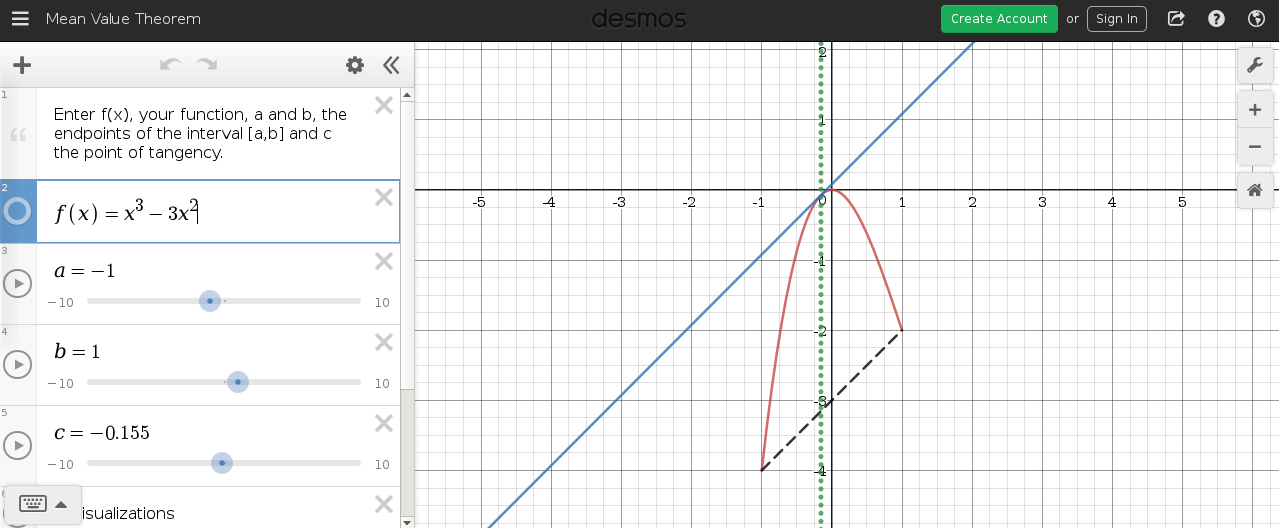
\includegraphics[width=\textwidth]{images/desmosDemo}
	\caption{Mean Value Theorem example that students can interact with}
\end{figure}
\begin{wrapfigure}{r}{0.35\textwidth}
	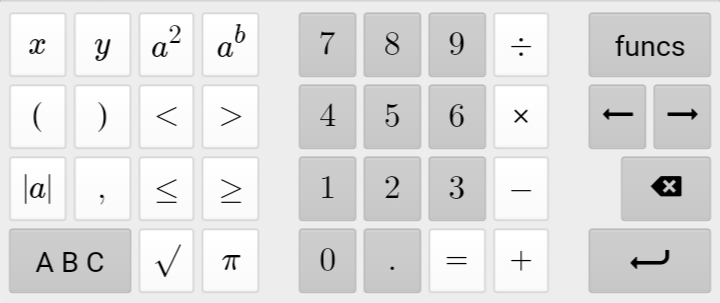
\includegraphics[width=0.35\textwidth]{images/desmosMobile}
	\caption{The Input}
\end{wrapfigure}
The problem however is that it is web based and as such, can be clunky to use. The mobile app and website are especially unresponsive when zooming in or out and when panning around. Another pitfall is that Desmos tries to make itself more secure in a way by restricting input. This however makes input very difficult to do and along with the unresponsiveness, it can be impossible to input the required equation.

On the other hand, the actual graph drawing is excellent, with many features such as inequalities, modulus functions and the ability to draw polar functions. It also highlights turning points, intersections with axes, inflection points and in the case of trigonometric functions, it expresses them in terms of $\pi$ instead of a numerical values.

Overall as a graphing calculator it does an excellent job, but has poor optimization issues and input, which I have realized are both important and need to be at the top of my list of requirements for my program.

In terms of other features, you can print, save and share your graphs to use later. I think that my program should have at least 1, if not all 3, of these features.

\section{GeoGebra}
GeoGebra is an interactive geometry, algebra, statistics and calculus application under the GNU General Public License, meaning that it is open source.

The main advantage to GeoGebra is that it can do a lot of things and is all of its features integrate well with each other. For example you can create a shape on the graph and create lines intersecting it, linking geometry with algebra. Individual line equations can also be moved around allowing for a very interactive experience. Like Desmos, you can create activities that you can interact with.

The mobile app for GeoGebra has a similar input to Desmos and as such suffers from the same problems. However it is more responsive than Desmos but only slightly. The desktop version however does not suffer from any of these problems.

As a pure graphing software, it does not automatically show the points of interest of a curve and is instead confined in a tool called the ``Function Inspector''. This tool is awkward to use as it only shows local maximums and minimums within a certain range (the highlighted red region), and if there are multiple roots, it does not acknowledge what the values of the roots are. Desmos does better than GeoGebra in this regard. Like Desmos it supports many functions that you can plot such as modulus and inequalities.
\begin{figure}[H]
	\begin{center}
		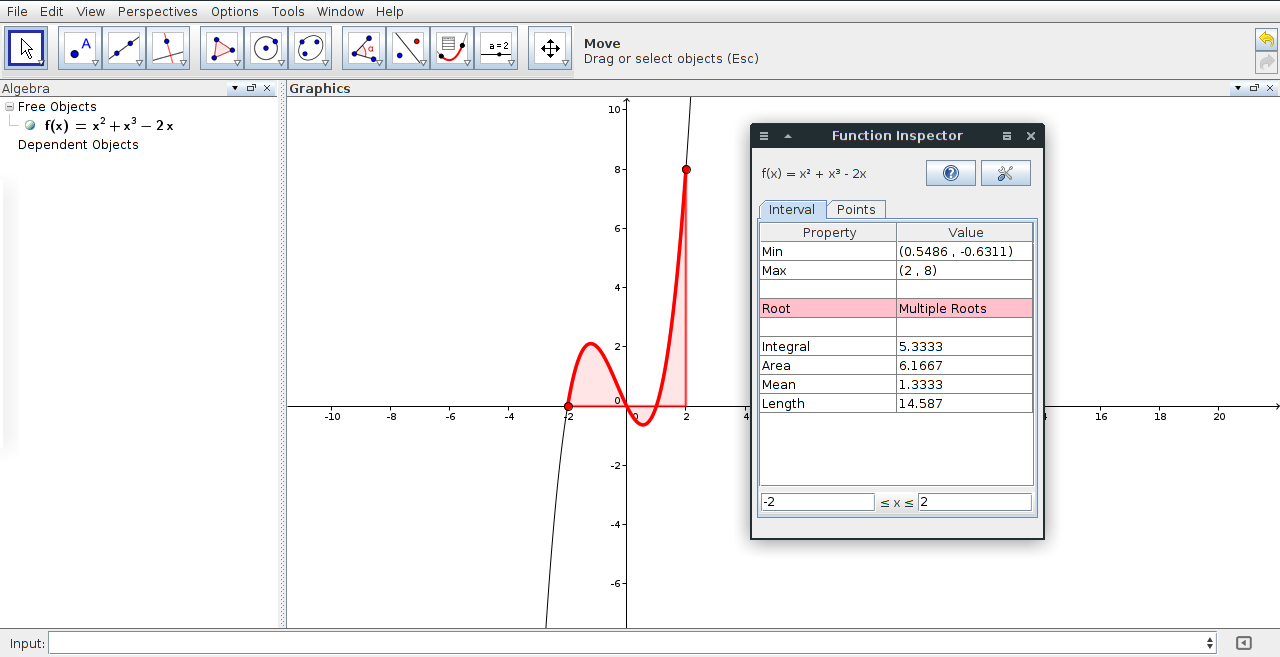
\includegraphics[width=0.77\textwidth]{images/geogebraFunc}
	\end{center}
	\caption{GeoGebra Function Inspector Tool}
\end{figure}
The panning and zooming in/out in GeoGebra is very fluid, with the zoom function being centered around the cursor. This means that you zoom in towards your cursor which feels more  responsive than if it zooms in/out from the center of the graph. The only criticism is that you can accidentally move already drawn graphs when trying to pan, which can be frustrating.

In terms of other features, like Desmos, you can save and print your work as well as being able to export it into other formats such as JPG, PNG or even convert it into a PSTricks or TikZ environment which can be used in \LaTeX \ documents for excellent graphs.

\section{GNU Octave}
GNU Octave is essentially an interpreter for a high level language centered around numerical calculation. GNU Octave is designed to be an open source software clone of MATLAB (MATrix LABatory).
\newline

Octave is different from GeoGebra and Desmos in the fact that it plots points that you tell it to not lines. For example if you wanted to plot $y=x^2$, you would define an array for your range in $x$ by doing:
\[x = -10:0.1:10;\]
This creates an array that starts at $-10$ increments by $0.1$ until $10$. You would then define $y$ by:
\[y = x.\wedge 2\]
You would then plot $x$ and $y$ by doing $plot(x,y);$.

As a graphing tool Octave is not very impressive, it has limited support for implicit functions and will not highlight points of interest of a curve. Realistically this is expected since Octave is primarily made for data presentation. This means that it can produce excellent plots, including meshes and surfaces
\footnote{A mesh is when a set of points in 3D space are joined up with lines to look like wire mesh. A surface is a mesh but adjacent points are used to make a solid shape instead, hence creating a surface.}
 in 3 dimensions.
\footnote{To clarify, a plot is where we explicitly define data that we then represent graphically, while a graph is where we define a relationship between 1 or more variables and represent this graphically.}
\begin{figure}[H]
\centering
\begin{minipage}{.7\textwidth}
	\centering
  	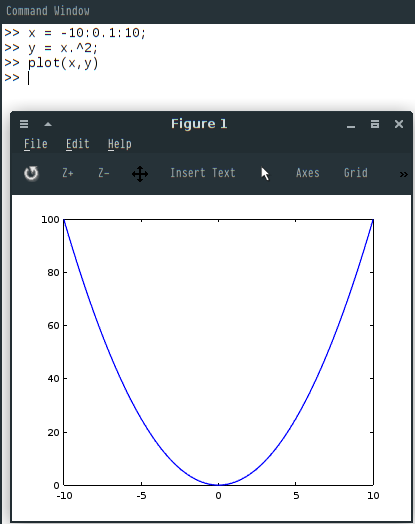
\includegraphics[width=0.3\textwidth]{images/octavePlot}
	\caption{Creating a simple plot in GNU Octave}
	\label{fig:octavePlot}
\end{minipage}%
\begin{minipage}{.3\textwidth}
	\centering
	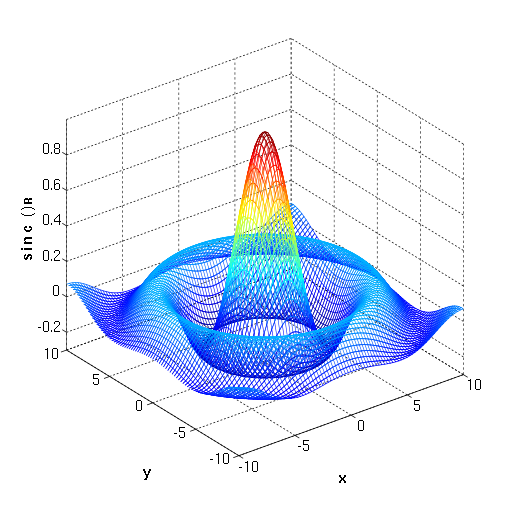
\includegraphics[width=0.65\textwidth]{images/matlabMesh}
	\caption{Wireframe 3D plot of the two-dimensional unnormalized sinc function}
\end{minipage}
\end{figure}
The way Octave plots (using the plot function at least) is by joining a line between consecutive points that it plots. I may use this in my program, since it seems more efficient to approximate a curve by making linear lines and joining them up than to check each pixel on the plot to check if it satisfies the given relation ship.

When inputting an algebraic expression in Octave it can be quite awkward, for example in Figure \ref{fig:octavePlot}, a period is before the carat. This is unnatural for us to input and as such can cause errors. Natural input is something that I think I should focus on since it is means that the program is easier to use and requires no further reading unlike Octave.

Octave is split into two views, the main editor view and a dockable plot view (you can also have multiple plots open at once). Dockable plots, or multiple plots could be something I implement later into my project.

Octave, like the other programs, can save plots and additionally the scripts you have made. It also has a feature that saves the current state when you close it, and resumes this state when you open it again. This could also be a feature I implement later into the project.

\section{Comparison}
Overall I think that I will be using aspects of all three of the programs that I have analyzed in my program. I think I should try and make my program as simple to use as Desmos. As mentioned, the input is a problem, and hence I will try and implement an input system like GeoGebras'. All three of the programs analyzed have some form of saving their plots, so I think that this is a feature that I should implement within my own program.

In terms of UI design, both Desmos and GeoGebra have a similar layout. They have an equation input box to the left, that can be minimized and the actual graph in the center left. I think that this layout is easy to use for the user so I will implement a similar design in my own program.

\begin{figure}[H]
	\begin{center}
		\includegraphics[width=0.9\textwidth]{diagrams/UI.mps}
	\end{center}
	\caption{UI Design}
\end{figure}

\end{document}